%%%%%%%%%%%%%%%%%%%%%%%%%%%%%%%%%%%%%%%%%
% Jacobs Landscape Poster
% LaTeX Template
% Version 1.1 (14/06/14)
%
% Created by:
% Computational Physics and Biophysics Group, Jacobs University
% https://teamwork.jacobs-university.de:8443/confluence/display/CoPandBiG/LaTeX+Poster
% 
% Further modified by:
% Nathaniel Johnston (nathaniel@njohnston.ca)
%
% This template has been downloaded from:
% http://www.LaTeXTemplates.com
%
% License:
% CC BY-NC-SA 3.0 (http://creativecommons.org/licenses/by-nc-sa/3.0/)
%
%%%%%%%%%%%%%%%%%%%%%%%%%%%%%%%%%%%%%%%%%


\documentclass[final]{beamer}
\usepackage[scale=1.24]{beamerposter}
\usetheme{confposter}

%-----------------------------------------------------------
% Define the column widths and overall poster size
% To set effective sepwid, onecolwid and twocolwid values, first choose how many columns you want and how much separation you want between columns
% In this template, the separation width chosen is 0.024 of the paper width and a 4-column layout
% onecolwid should therefore be (1-(# of columns+1)*sepwid)/# of columns e.g. (1-(4+1)*0.024)/4 = 0.22
% Set twocolwid to be (2*onecolwid)+sepwid = 0.464
% Set threecolwid to be (3*onecolwid)+2*sepwid = 0.708

\newlength{\sepwid}
\newlength{\onecolwid}
\newlength{\twocolwid}
\newlength{\threecolwid}
\setlength{\paperwidth}{48in} % A0 width: 46.8in
\setlength{\paperheight}{36in} % A0 height: 33.1in
\setlength{\sepwid}{0.024\paperwidth} % Separation width (white space) between columns
\setlength{\onecolwid}{0.22\paperwidth} % Width of one column
\setlength{\twocolwid}{0.464\paperwidth} % Width of two columns
\setlength{\threecolwid}{0.708\paperwidth} % Width of three columns
\setlength{\topmargin}{-0.5in} % Reduce the top margin size
%-----------------------------------------------------------

\usepackage{graphicx}
\usepackage{booktabs}
\title{Stimulus Identification from fMRI scans}

\author{Charles Zheng and Yuval Benjamini} % Author(s)

\institute{Stanford University, Department of Statistics} % Institution(s)

%----------------------------------------------------------------------------------------

\begin{document}

\addtobeamertemplate{block end}{}{\vspace*{2ex}} % White space under blocks
\addtobeamertemplate{block alerted end}{}{\vspace*{2ex}} % White space under highlighted (alert) blocks

\setlength{\belowcaptionskip}{2ex} % White space under figures
\setlength\belowdisplayshortskip{2ex} % White space under equations

\begin{frame}[t] % The whole poster is enclosed in one beamer frame

\begin{columns}[t] % The whole poster consists of three major columns, the second of which is split into two columns twice - the [t] option aligns each column's content to the top

\begin{column}{\sepwid}\end{column} % Empty spacer column

\begin{column}{\onecolwid} % The first column

%----------------------------------------------------------------------------------------
%	INTRODUCTION
%----------------------------------------------------------------------------------------

\setbeamercolor{block alerted title}{fg=white,bg=Violet} % Change the alert block title colors
\setbeamercolor{block alerted body}{fg=black,bg=white} % Change the alert block body colors

\begin{alertblock}{Overview}
\vspace{0.3in}

Seeking to explain the processes behind human perception, scientists
employ \emph{forward models} to model the causal relationship between
stimulus and neural activity.  But how can we measure the quality of
these models?  Kay et al (2008) introduced the
task of \emph{identification} as a way to demonstrate the fidelity and
generalizability of the model.
\vspace{0.7in}

Using the data of Kay \emph{et al.} as a motivating example, we
consider the statistical problem of optimal identification.  While
identification superficially resembles a classification task (with
many classes), it combines the challenge of multivariate regression
with high-dimensional discrimination.
\end{alertblock}

\begin{block}{Data}
\begin{itemize}
\item Sequence of stimuli (pictures) shown at time $t = 1,\hdots, T = 3500$
\item Record subject's multivariate response $Y_t \in \mathbb{R}^p$, here $p \approx 20000$
\end{itemize}

\begin{center}
\begin{tabular}{ccccc}
$t = 1$ & $t = 2$ & $t = 3$ & $t = 4$ & $\cdots$\\ \hline
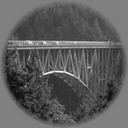
\includegraphics[scale = 0.5]{img1.png} &
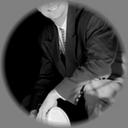
\includegraphics[scale = 0.5]{img2.png} &
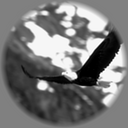
\includegraphics[scale = 0.5]{img3.png} &
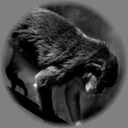
\includegraphics[scale = 0.5]{img4.png} & $\cdots$\\ \hline
$Y_1$ & $Y_2$ & $Y_3$ & $Y_4$ & $\cdots$\\ \hline
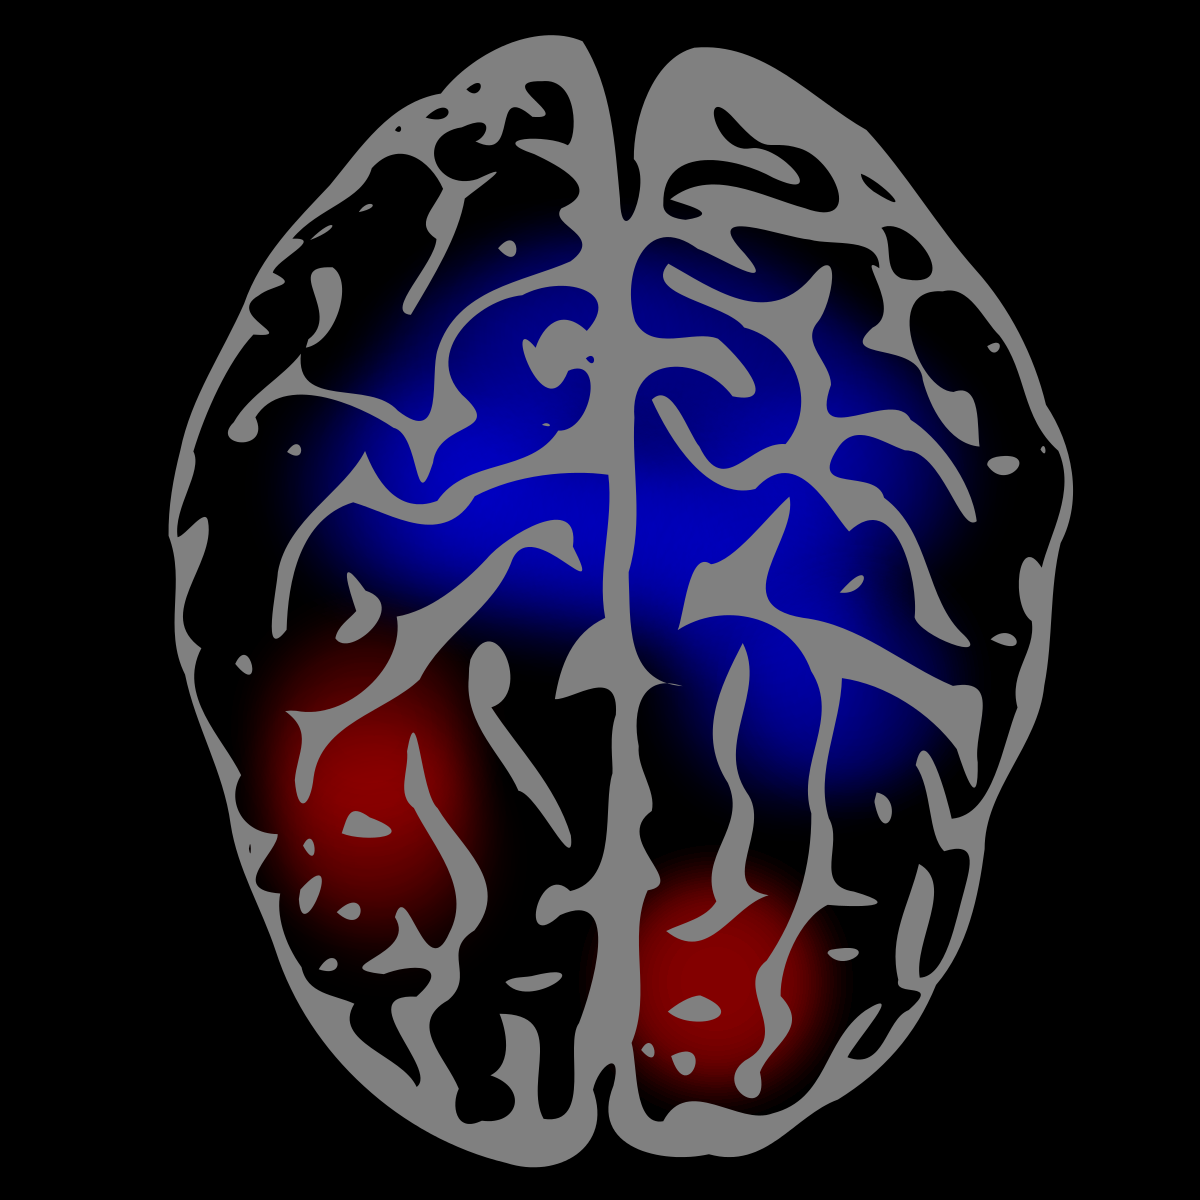
\includegraphics[scale = 0.06]{brain1.png} &
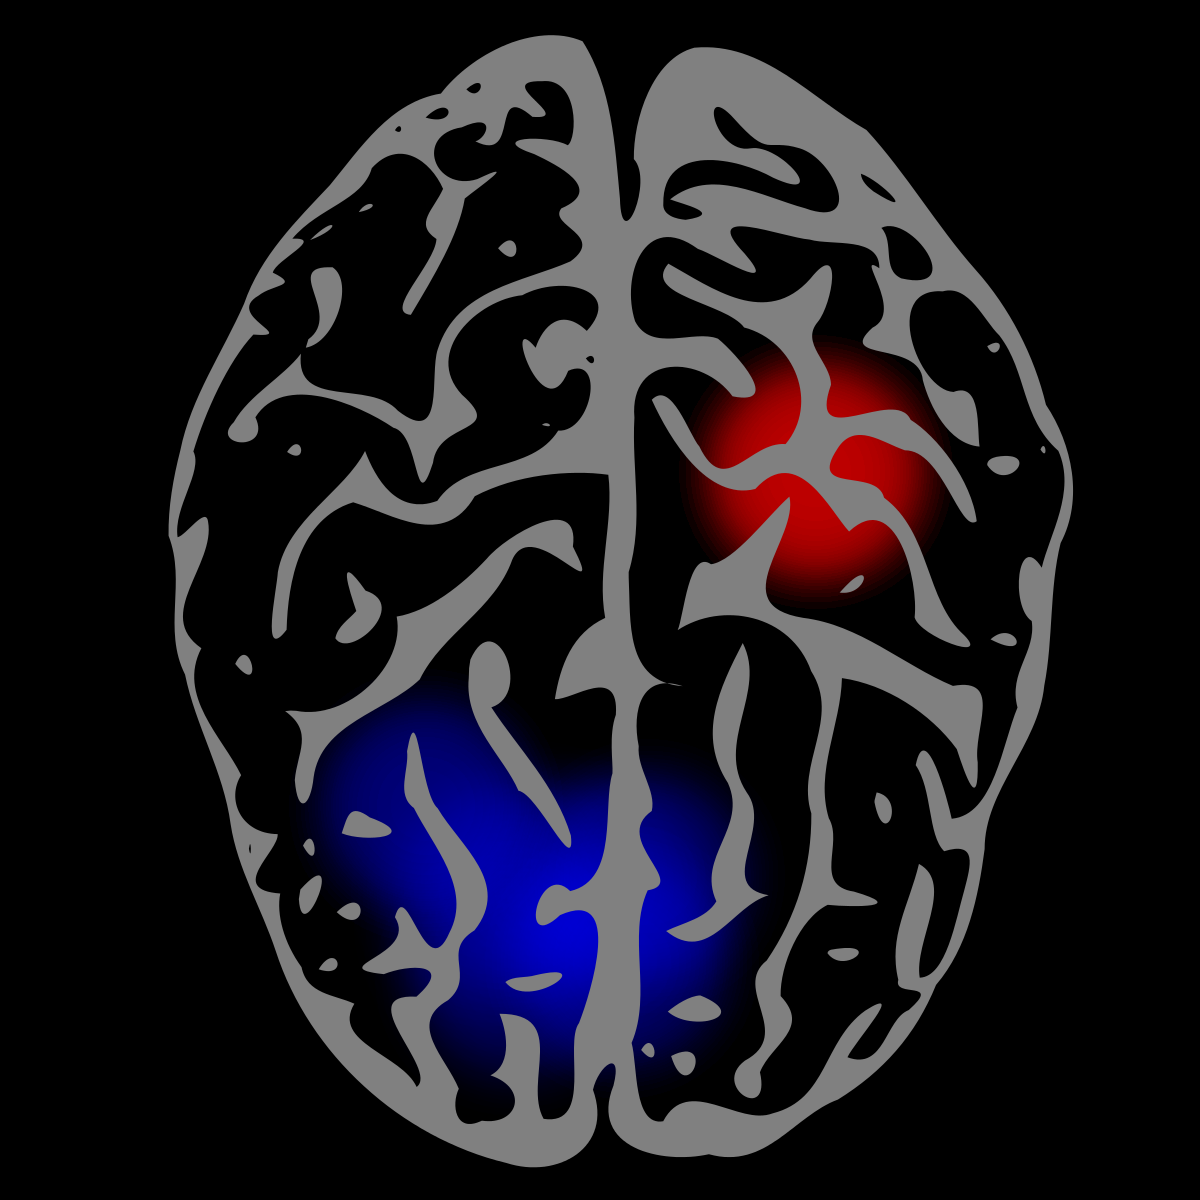
\includegraphics[scale = 0.06]{brain2.png} &
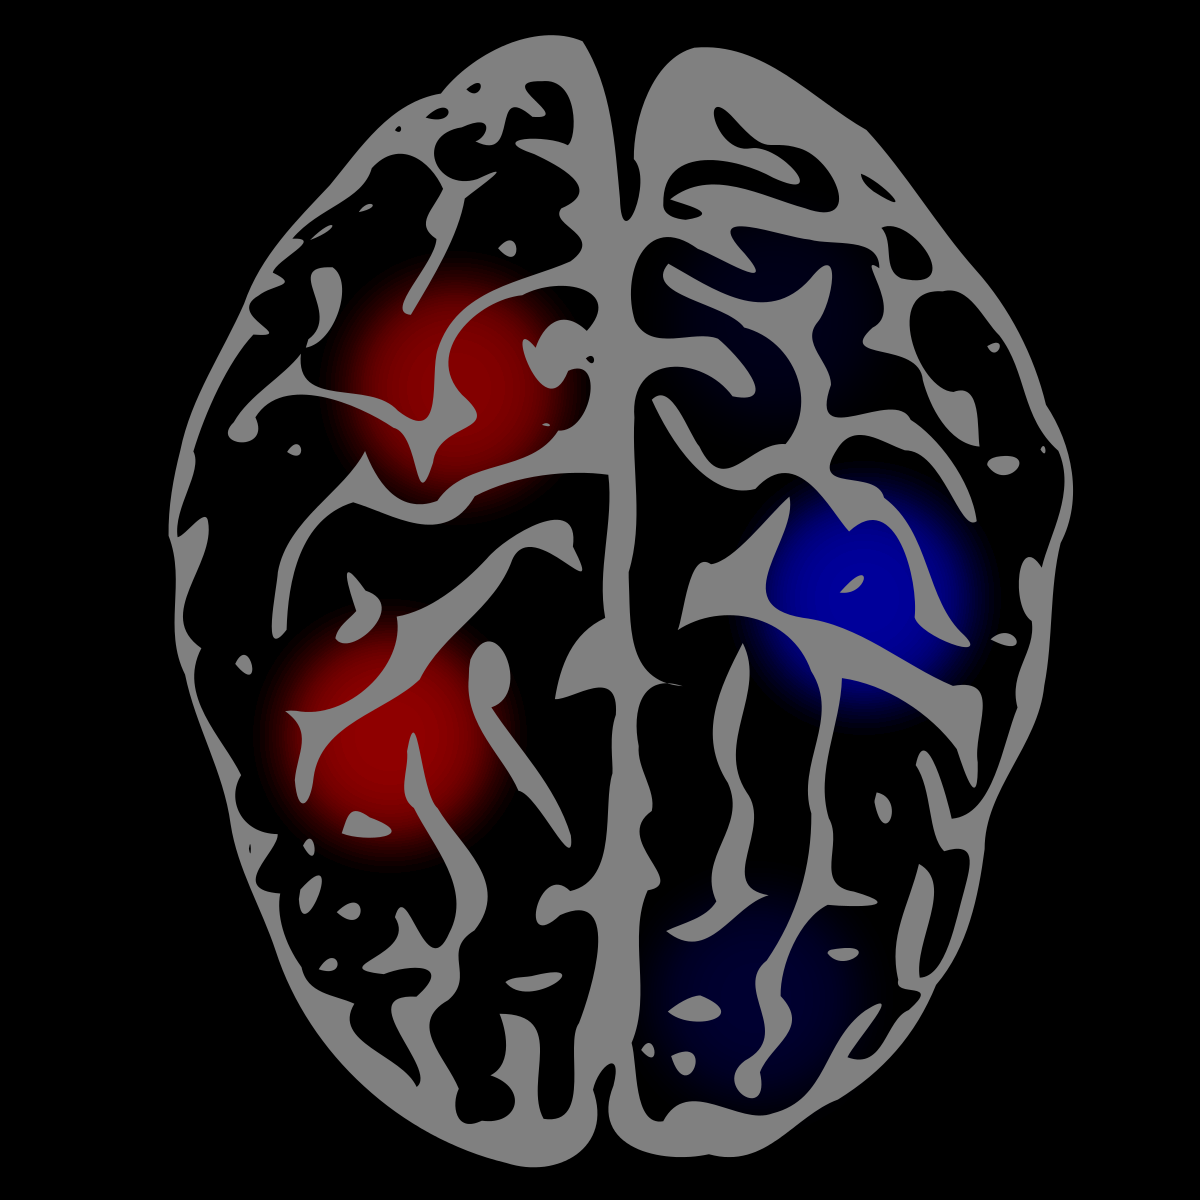
\includegraphics[scale = 0.06]{brain3.png} &
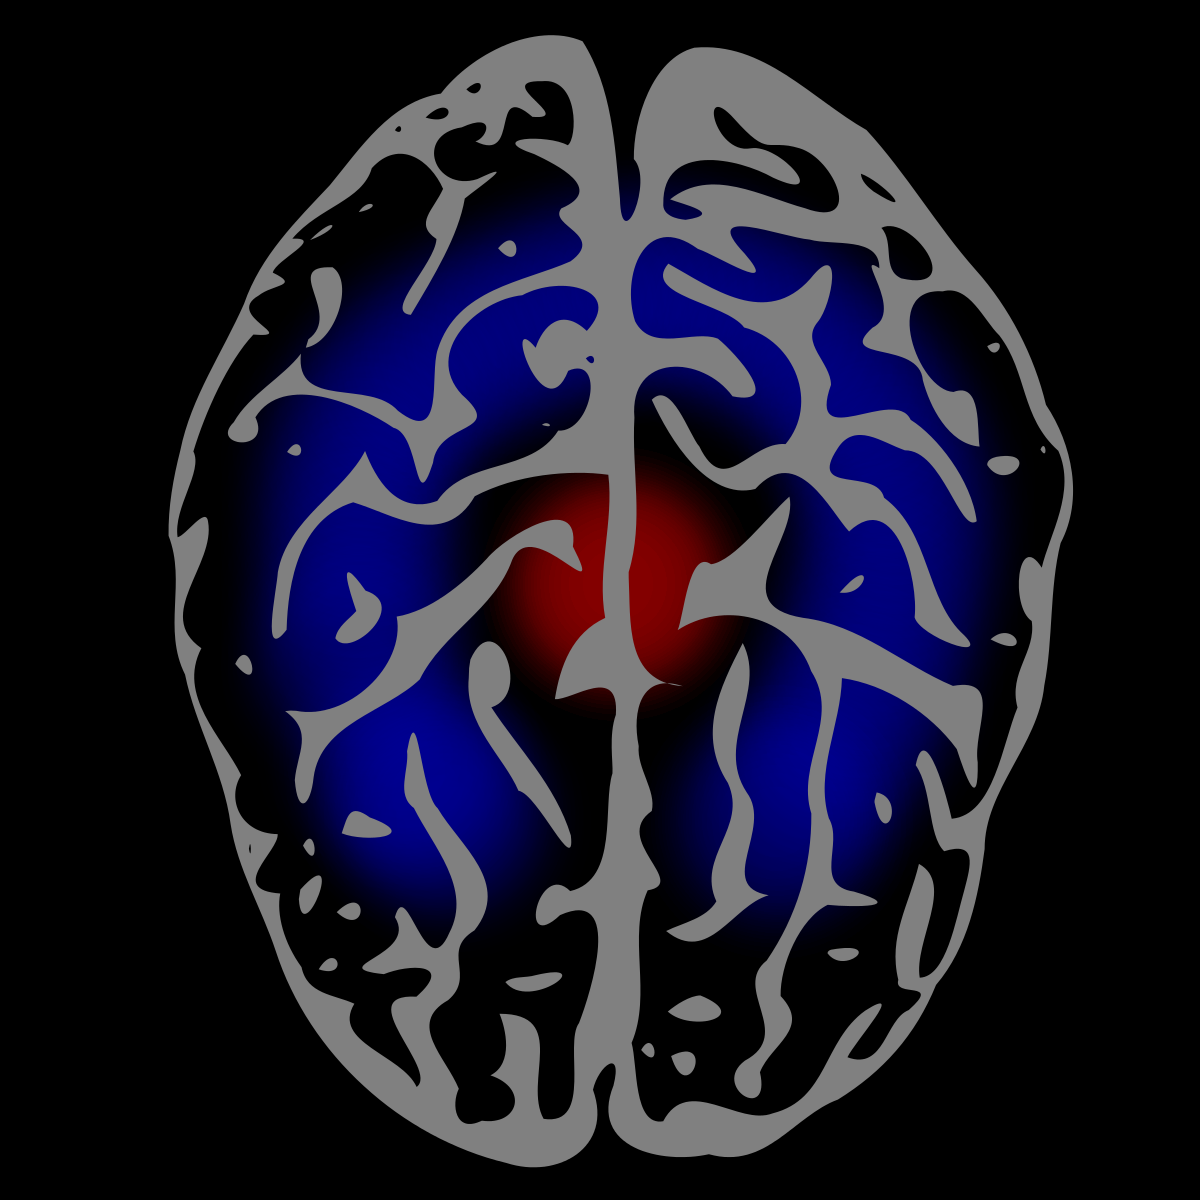
\includegraphics[scale = 0.06]{brain4.png} & $\cdots$\\ \hline
\end{tabular}
\end{center}
\end{block}



%\begin{itemize}
%\item Stimuli represented as \emph{feature vector} $X_t \in \mathbb{R}^q$
%\item Linear model:
%\[
%
%\]
%\item E.g. Kay (2008)
%\end{itemize}


\begin{block}{Identification}
\begin{center}
\begin{tabular}{c|c|cccc}
\hline
$y^*$ &     & &  $i^* = ?$  &   \\
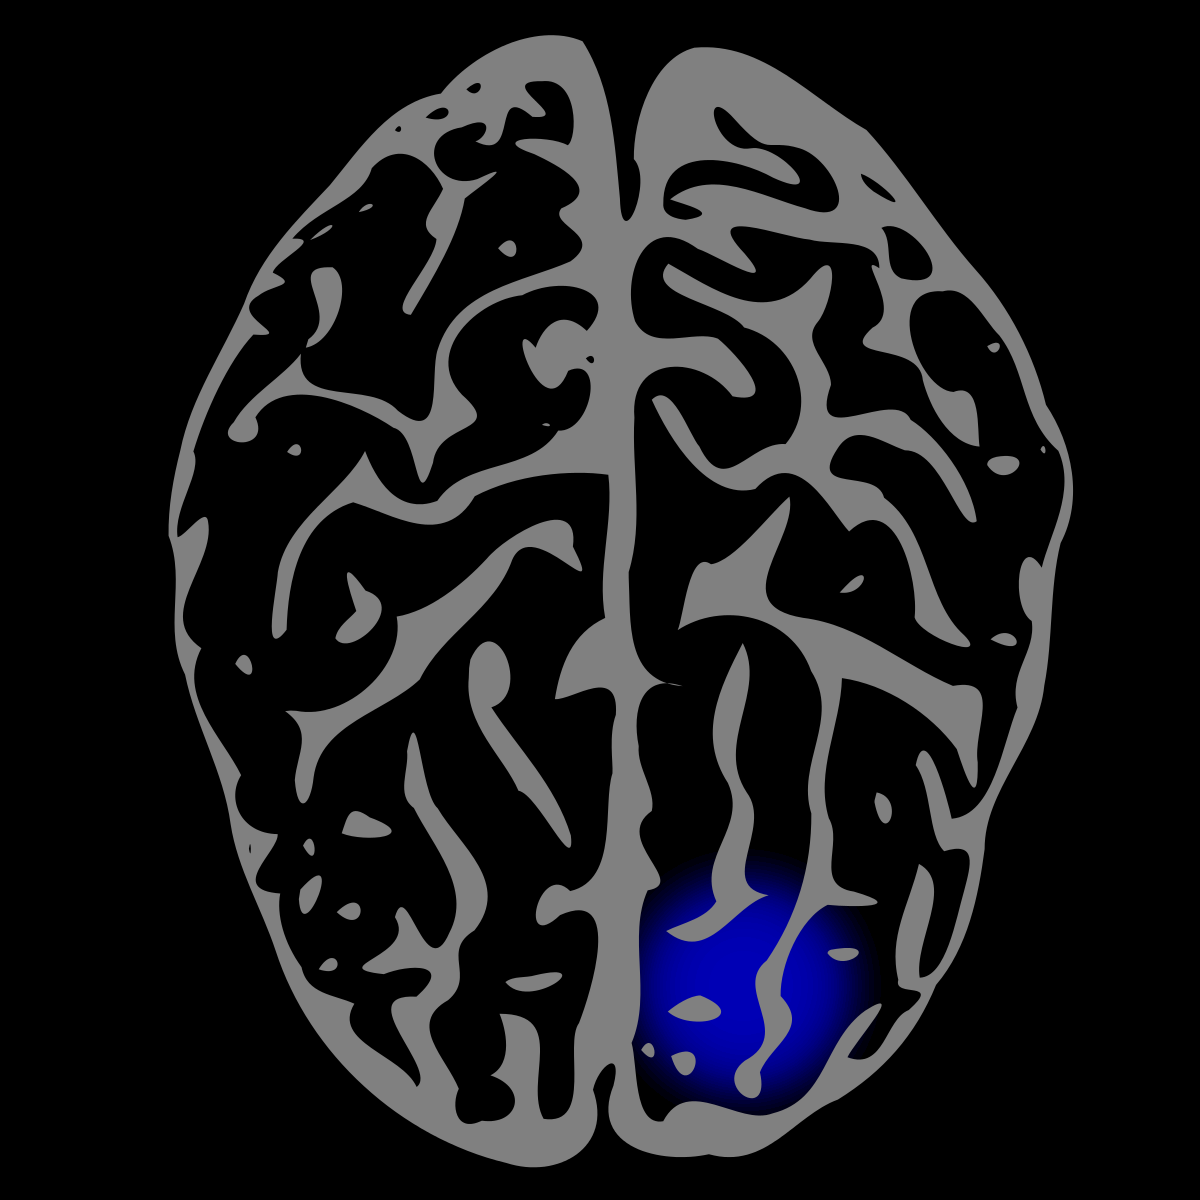
\includegraphics[scale = 0.06]{brain7.png} & \hspace{0.5in} 
& 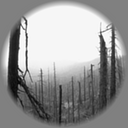
\includegraphics[scale = .5]{img5.png}
& 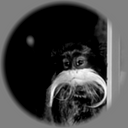
\includegraphics[scale = .5]{img6.png}
& 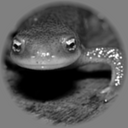
\includegraphics[scale = .5]{img7.png}
& 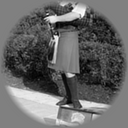
\includegraphics[scale = .5]{img8.png}\\
\hline
\end{tabular}
\end{center}
\begin{itemize}
\item Let $S$ be a set of \emph{new} stimuli--no repeats from the training set!  Here $|S| = 120$.
\item Scientist picks a stimulus $i^*$ from $S$ and measures the subject's reponse $y^*$
\item Can the statistician \emph{identify} $i^* \in S$ from $y^*$?
\end{itemize}
\end{block}

\end{column} % End of the first column

\begin{column}{\sepwid}\end{column} % Empty spacer column



\begin{column}{\onecolwid}

%----------------------------------------------------------------------------------------
%	MATERIALS
%----------------------------------------------------------------------------------------



\begin{block}{Previous Work}

Kay (2008) and Vu (2011) reduce the dimensionality of $Y$ (by applying
a filter based on SNR) and consider a linear model
\[
Y_{T \times p} = X_{T \times q} B_{q \times p} + E_{T \times p}
\]
where $X$ are a set of \emph{image features} (Gabor filters), $q \approx 10000$.

They identify the stimuli based on the \emph{maximum likelihood} (ML) principle:

\begin{itemize}
\item Obtain point estimates of coefficients $B$ and noise covariance $\Sigma_E$
\item E.g. $B$ estimated using elastic net with CV (Zou 2005),
shrinkage estimate for covariance
\[
\hat{\Sigma}_E = \frac{1}{2}\hat{\text{Cov}}(Y - \hat{Y}) + \frac{1}{2}\text{diag}(\hat{\text{Cov}}(Y - \hat{Y}))
\]
where $\hat{\text{Cov}}$ denotes sample covariance
\item Obtain predicted means for test stimuli
\[
\hat{\mu}_i^{te} = (x_i^{te})^T B
\]
\item Identify the stimulus $i^*$ by
\[
i^* = \text{argmin}_{i} (\hat{\mu}_i^{te} - y^*)^T \hat{\Sigma}_E^{-1} (\hat{\mu}_i^{te} - y^*)
\]
\end{itemize}
\end{block}

\begin{block}{Limitations of ML}
\begin{itemize}
\item Estimation of $B$ are motivated by \emph{prediction error}: the loss function for identification is different!
\item \emph{Fact:} Any estimate of $B$ which is degenerate (low-rank) is suboptimal
\end{itemize}
\begin{center}
\begin{tabular}{ccc}
(a) & (b) & (c)\\
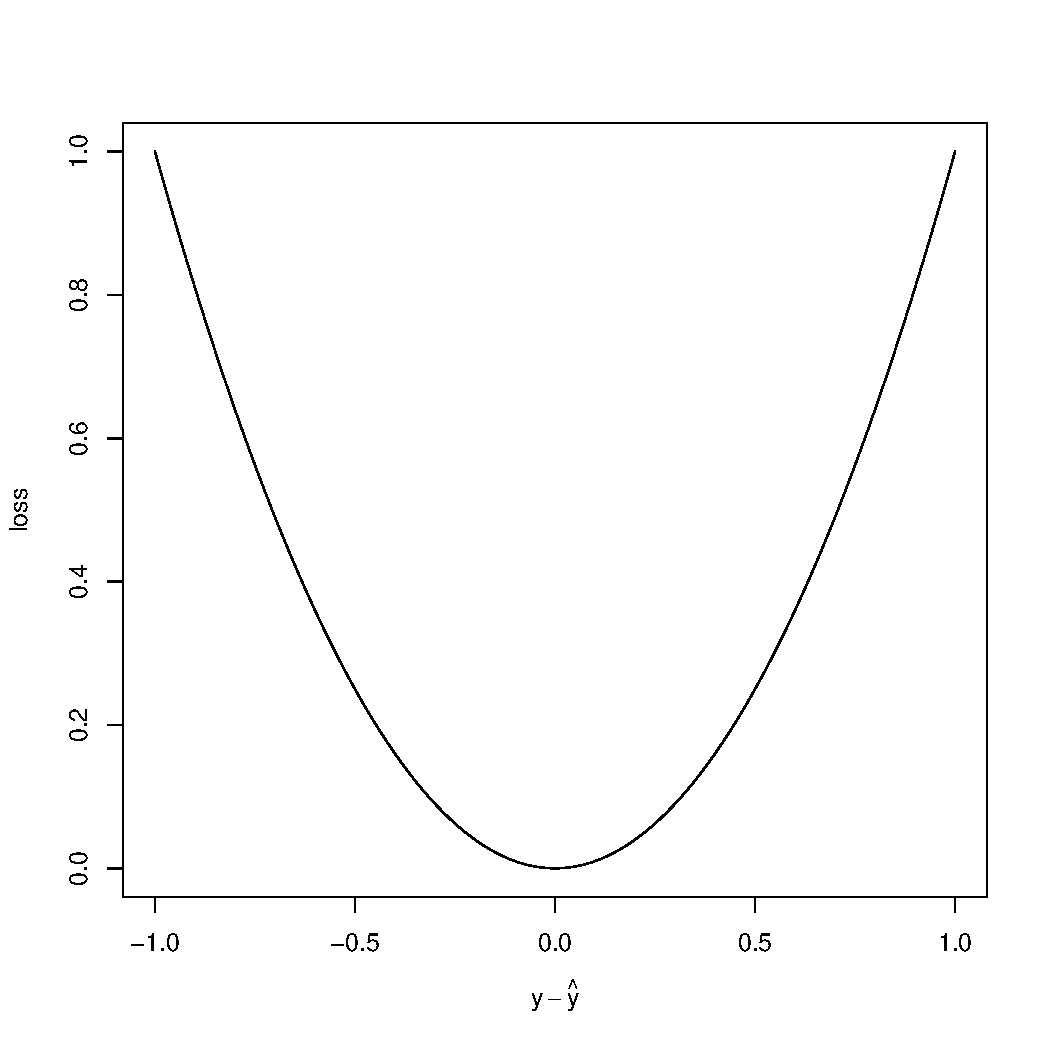
\includegraphics[scale = 0.5, trim = 1in 1in 0.5in 1in, clip]{loss_se.pdf} & 
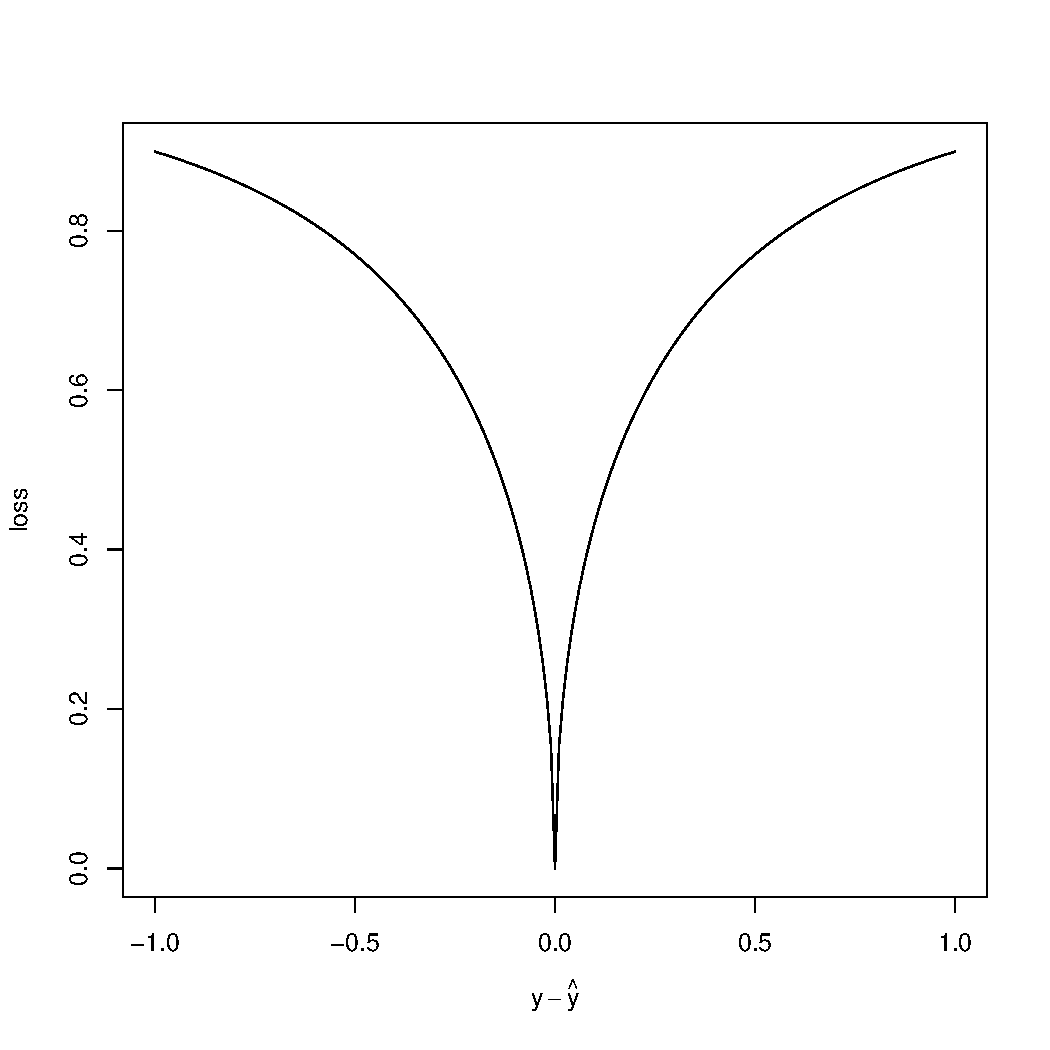
\includegraphics[scale = 0.5, trim = 1in 1in 0.5in 1in, clip]{loss_3.pdf} &
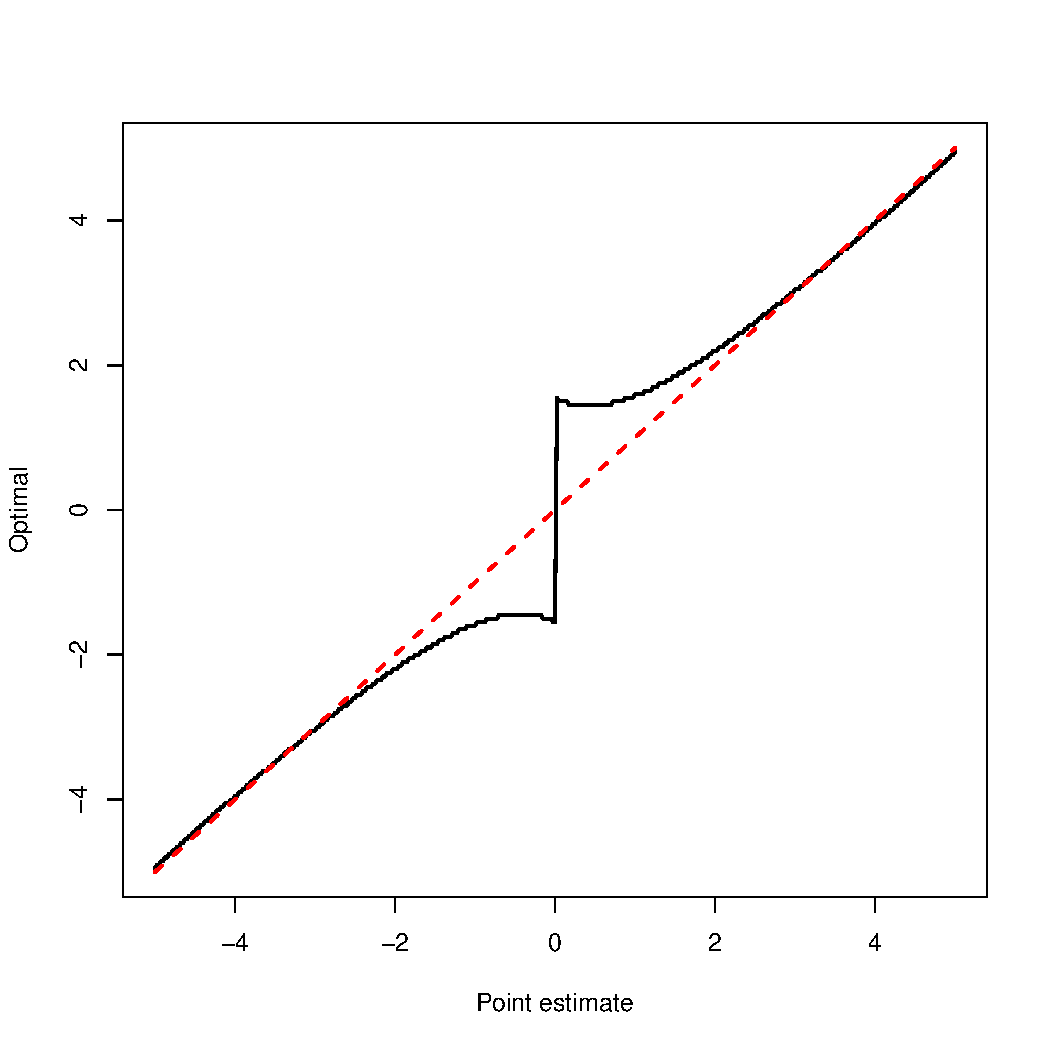
\includegraphics[scale = 0.5, trim = 1in 1in 0.5in 1in, clip]{zero2.pdf}\\
{\small 0} & {\small 0} & {\small 0}\\
\end{tabular}
\end{center}
{\small
\emph{(a)} Squared error loss (vertical axis) and \emph{(b)} loss function for identification,
as a function of the difference between the true mean signal and the predicted signal.\\
\emph{(c)} The optimal point estimate for identification (solid) vs the optimal point estimate for regression (dashed)
diverge sharply at 0 in the one-dimensional case.  ($B = 0$ a special case of degenerate $B$)
}
\end{block}

%\begin{center}
%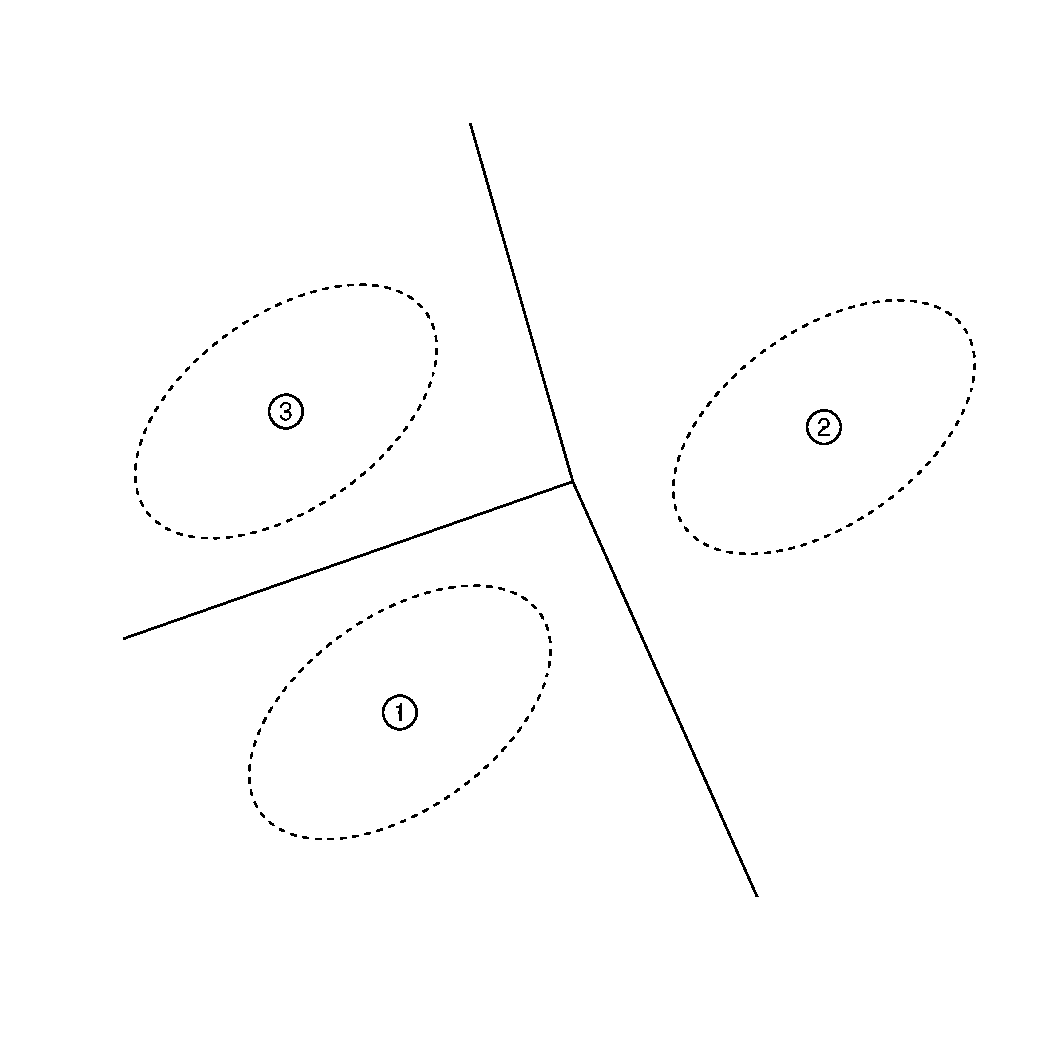
\includegraphics[scale = 1.0]{illus1_A.pdf}
%\end{center}

%\emph{Theoretical results}
%\begin{itemize}
%\item Asymptotic consistency to optimal procedure $T \to \infty$ under correct model specification
%\item Inconsistency given model misspecification (nonlinearity)
%\end{itemize}



%----------------------------------------------------------------------------------------

\end{column} % End of column 2.1

\begin{column}{\sepwid}\end{column} % Empty spacer column


\begin{column}{\onecolwid}

\begin{block}{Empirical Bayes}

\begin{itemize}
\item 
\emph{Proposal}: improve on ML by accounting for the uncertainty of the
estimate $B$.
\item We consider a hierarchical model with a prior
distribution on $B$, but we use the data to set the prior covariance
$\Sigma_B$--hence we are being \emph{empirical Bayesians}
\item In contrast to ML, which results in \emph{linear decision
  boundaries} (below: left), Empirical Bayes (EB) results in \emph{quadratic boundaries} (below: right)
\end{itemize}

\begin{center}
\begin{tabular}{cc}
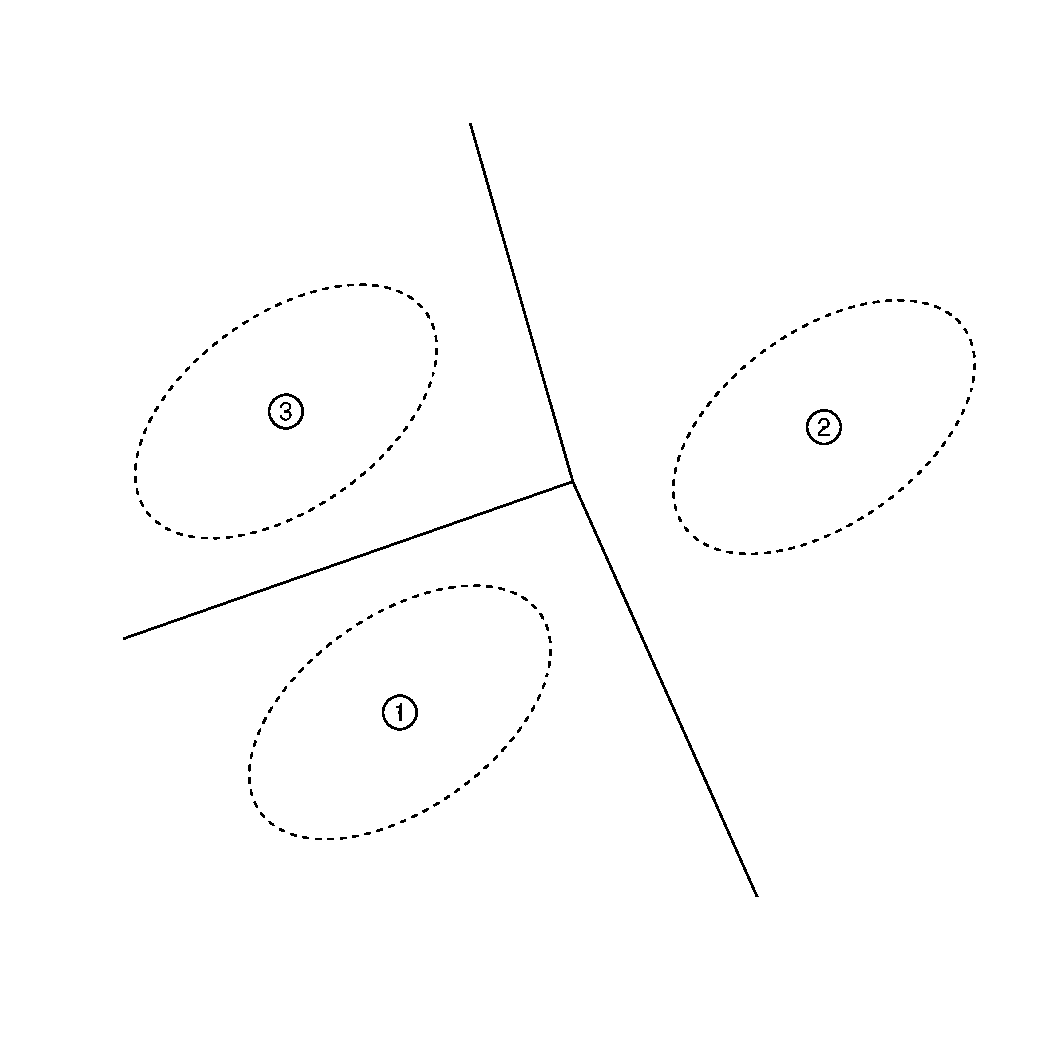
\includegraphics[scale = 0.5]{illus1_A.pdf} & 
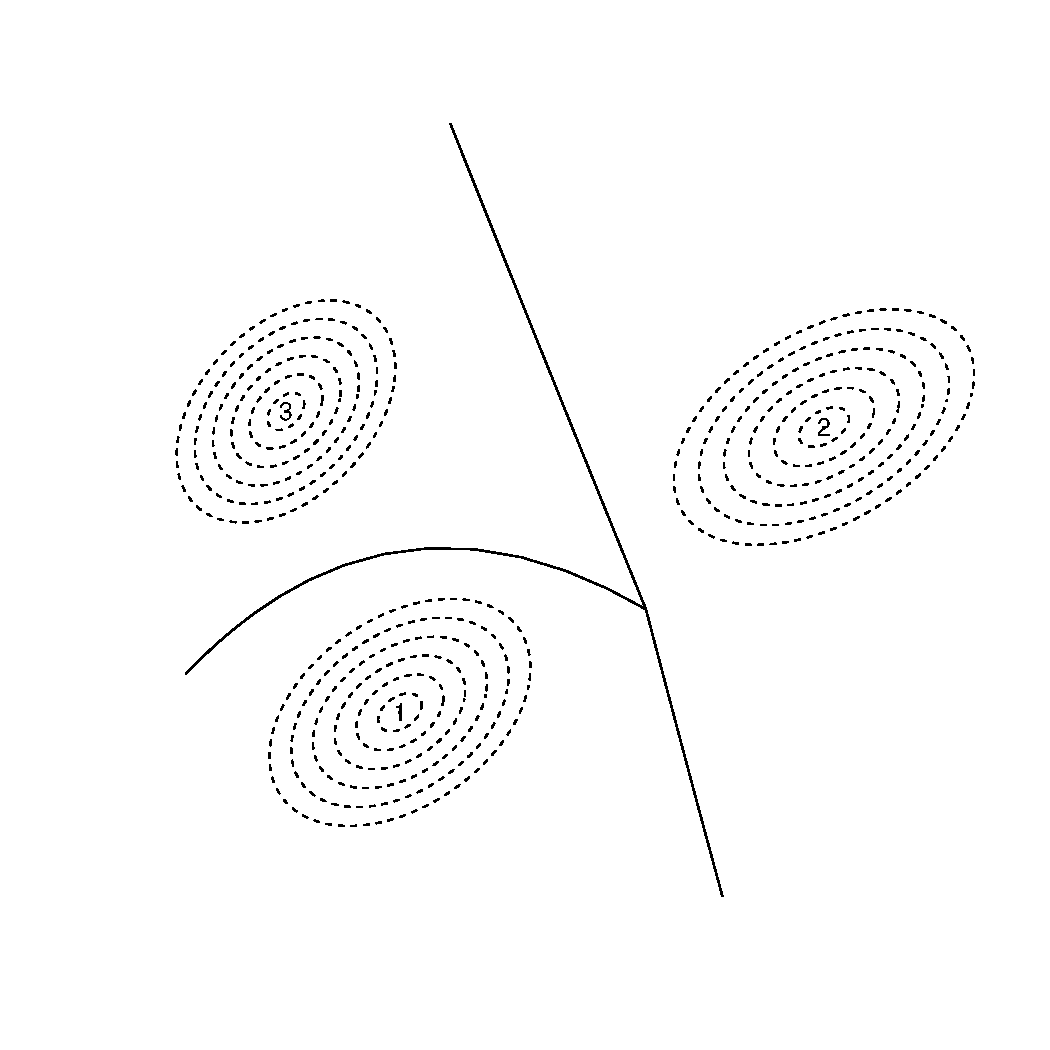
\includegraphics[scale = 0.5]{illus1_B.pdf}\\
ML & EB
\end{tabular}
\end{center}
\end{block}

\begin{alertblock}{Technical details}
\emph{Model}

\begin{itemize}
\item Noise $E_t \sim N(0, \Sigma_E)$ iid 
\item Coefficients $B_i \sim N(0, \sigma^2_i I)$ for $i = 1, \hdots, p$
\item $X$ non-random
\end{itemize}

\emph{Estimate hyperparameters}

\begin{itemize}
\item Use \emph{eigenprism} (Janson 2015) to estimate $\theta_i^2 = ||B_i||^2$ for $i =1,\hdots, p$
\item Set $\sigma^2_i = \hat{\theta}_i^2/q$
\item Estimate $\hat{B}$ as posterior mean
\item Estimate $\Sigma_E$ (same as in ML)
\end{itemize}

\emph{Compute posterior}
\begin{itemize}
\item Closed-form expressions for posteriors of $B$, $\mu_i^{te}$
\item Computational bottleneck: inverting a $pq \times pq$ covariance matrix
\end{itemize}

\emph{Apply Bayes rule}

\begin{itemize}
\item \emph{Uncertainty} in $B$ is reflected as \emph{added noise}
\item Result: posterior $\text{Cov}(y^*|i^*)$ varies, hence \emph{quadratic boundaries}
\end{itemize}

\end{alertblock}


%----------------------------------------------------------------------------------------

\end{column} % End of column 2.2

\begin{column}{\sepwid}\end{column} % Empty spacer column

\begin{column}{\onecolwid} % The third column

%----------------------------------------------------------------------------------------
%	CONCLUSION
%----------------------------------------------------------------------------------------

\begin{block}{Simulation Results}
\begin{itemize}
\item Parameters $p = q = 60$, random coefficients
\item Empirical bayes outperforms ML when $n < q$... however, still unstable!
\end{itemize}
\begin{center}
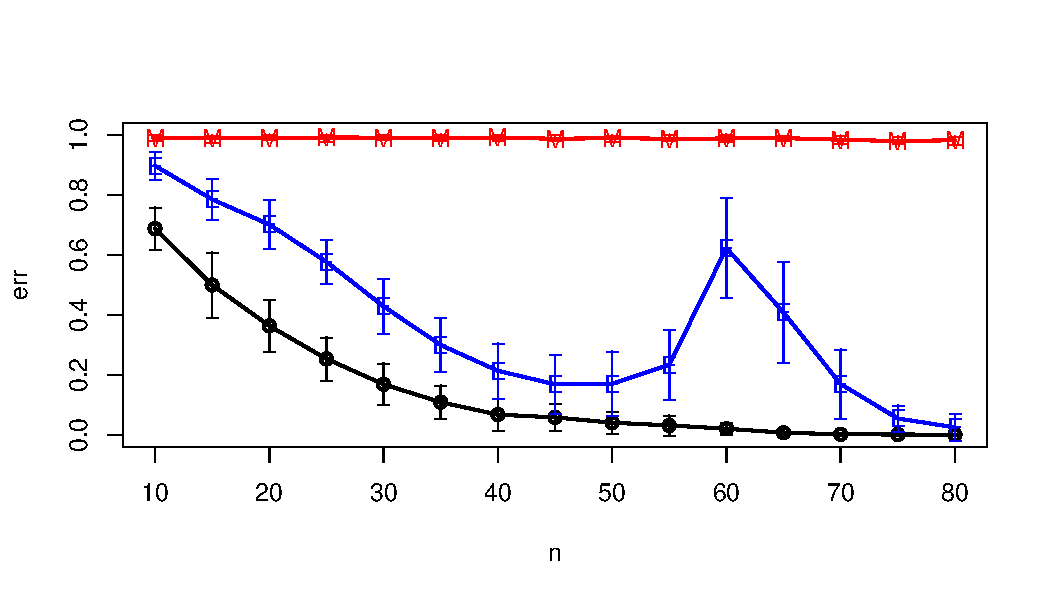
\includegraphics[scale = 1.3]{simulation1.pdf}
\end{center}
\small{
 \textcolor{blue}{(E)} Empirical Bayes,  \textcolor{red}{(M)} Maximum likliehood,
(o) Bayes risk \emph{(knowing true $\Sigma_B$, $\Sigma_E$)}}
\end{block}

\begin{block}{Ongoing Work}
\begin{itemize}
\item Why does error \emph{increase} with sample size!? Refine covariance estimation methods..
\item Required cost of $O((pq)^3)$ unacceptable for real data... develop tractable approximations
\item Apply methods to data of Kay (2008)
\end{itemize}
\end{block}

\setbeamercolor{block alerted title}{fg=white,bg=Violet} % Change the alert block title colors
\setbeamercolor{block alerted body}{fg=black,bg=white} % Change the alert block body colors

\begin{block}{Conclusions}
\begin{itemize}
\item We determine theoretical limitations of Maximum Likelihood, and
  illustrate the promise of Empirical Bayes... but our own method
  still has obvious flaws
\item Many challenges remain for optimal identification!
\end{itemize}
\end{block}

%----------------------------------------------------------------------------------------
%	REFERENCES
%----------------------------------------------------------------------------------------

\begin{block}{References}


\small{
\begin{itemize}
\item Kay et al. \emph{Nature} (2008)
\item Vu et al. \emph{Annals of Applied Statistics} (2011)
\item Janson et al. (2015) http://arxiv.org/abs/1505.02097
\end{itemize}
}

\end{block}

%----------------------------------------------------------------------------------------
%	ACKNOWLEDGEMENTS
%----------------------------------------------------------------------------------------

\begin{block}{Acknowledgements}


\small{ This work was supported by an NSF graduate research fellowship.
  We are also grateful to the travel support provided by the SAND 7 conference.  }

\end{block}




%----------------------------------------------------------------------------------------

\end{column} % End of the third column

\end{columns} % End of all the columns in the poster

\end{frame} % End of the enclosing frame

\end{document}
